% !TEX root = ../main.tex
\chapter{Progettazione della base di dati}
\label{cap:database}

\section{Modello Entità-Relazione}

La base di dati persiste le entità principali del dominio in una struttura relazionale formata da utenti (\texttt{USER}), venue (\texttt{VENUE}), risorse logiche e fisiche (\texttt{SPACE}, \texttt{EQUIPMENT}, \texttt{SERVICE}), eventi (\texttt{EVENT}), richieste di evento (\texttt{EVENT\_REQUEST}), prenotazioni (\texttt{BOOKING}), biglietti (\texttt{TICKET}), ospiti (\texttt{EVENT\_GUEST}), recensioni (\texttt{REVIEW}) e report (\texttt{REPORT}). Le relazioni molti-a-molti tra le entità sono gestite tramite tabelle di associazione appositamente implementate.

L'entità \texttt{USER} rappresenta sia gli utenti standard sia gli amministratori: il ruolo amministrativo è memorizzato nell'attributo \texttt{is\_admin}, invece che in una tabella separata. L'utente ricopre ruoli differenti nelle relazioni con gli eventi e le richieste: può essere creatore e organizzatore per un evento, e richiedente e gestore per una richiesta. L'entità \texttt{VENUE} è collegata agli eventi e alle richieste e contiene gli spazi (\texttt{SPACE}), oltre a poter essere associata alle attrezzature (\texttt{EQUIPMENT}); i servizi (\texttt{SERVICE}) sono invece globali e non sono legati direttamente a una venue specifica.

Nello schema non è definita una relazione diretta tra \texttt{EVENT} ed \texttt{EVENT\_REQUEST}: una richiesta accettata non è collegata tramite chiave esterna a un evento eventualmente creato in seguito. In maniera analoga, \texttt{EVENT\_GUEST} rappresenta un ospite invitato e non richiede un account \texttt{USER}; \texttt{Address} non possiede una tabella a sé, e i campi dell'indirizzo sono memorizzati direttamente all'interno di \texttt{VENUE}.

Le associazioni tra eventi o richieste e spazi, attrezzature e servizi possiedono tabelle specifiche; tra queste, le associazioni con attrezzature e servizi includono l'attributo \texttt{quantity}, mentre quelle relative agli spazi non possiedono attributi propri. \texttt{BOOKING} collega un utente a un evento e \texttt{TICKET} rappresenta un biglietto nominativo collegato a una specifica prenotazione. \texttt{REVIEW} collega un utente a un evento, mentre \texttt{REPORT} collega due utenti (un amministratore e un utente segnalato) e può anche riferirsi facoltativamente a un evento.

Le cardinalità concettuali del modello non sono sempre tradotte totalmente tramite le chiavi esterne dello schema relazionale. Infatti, le FK impongono la coerenza dei riferimenti verso le tabelle padre, mentre il rispetto delle molteplicità minime richieste dalle regole di business viene garantito dai controlli applicativi, come illustrato più nel dettaglio nella sezione sui vincoli.

\begin{figure}[!htbp]
    \centering
    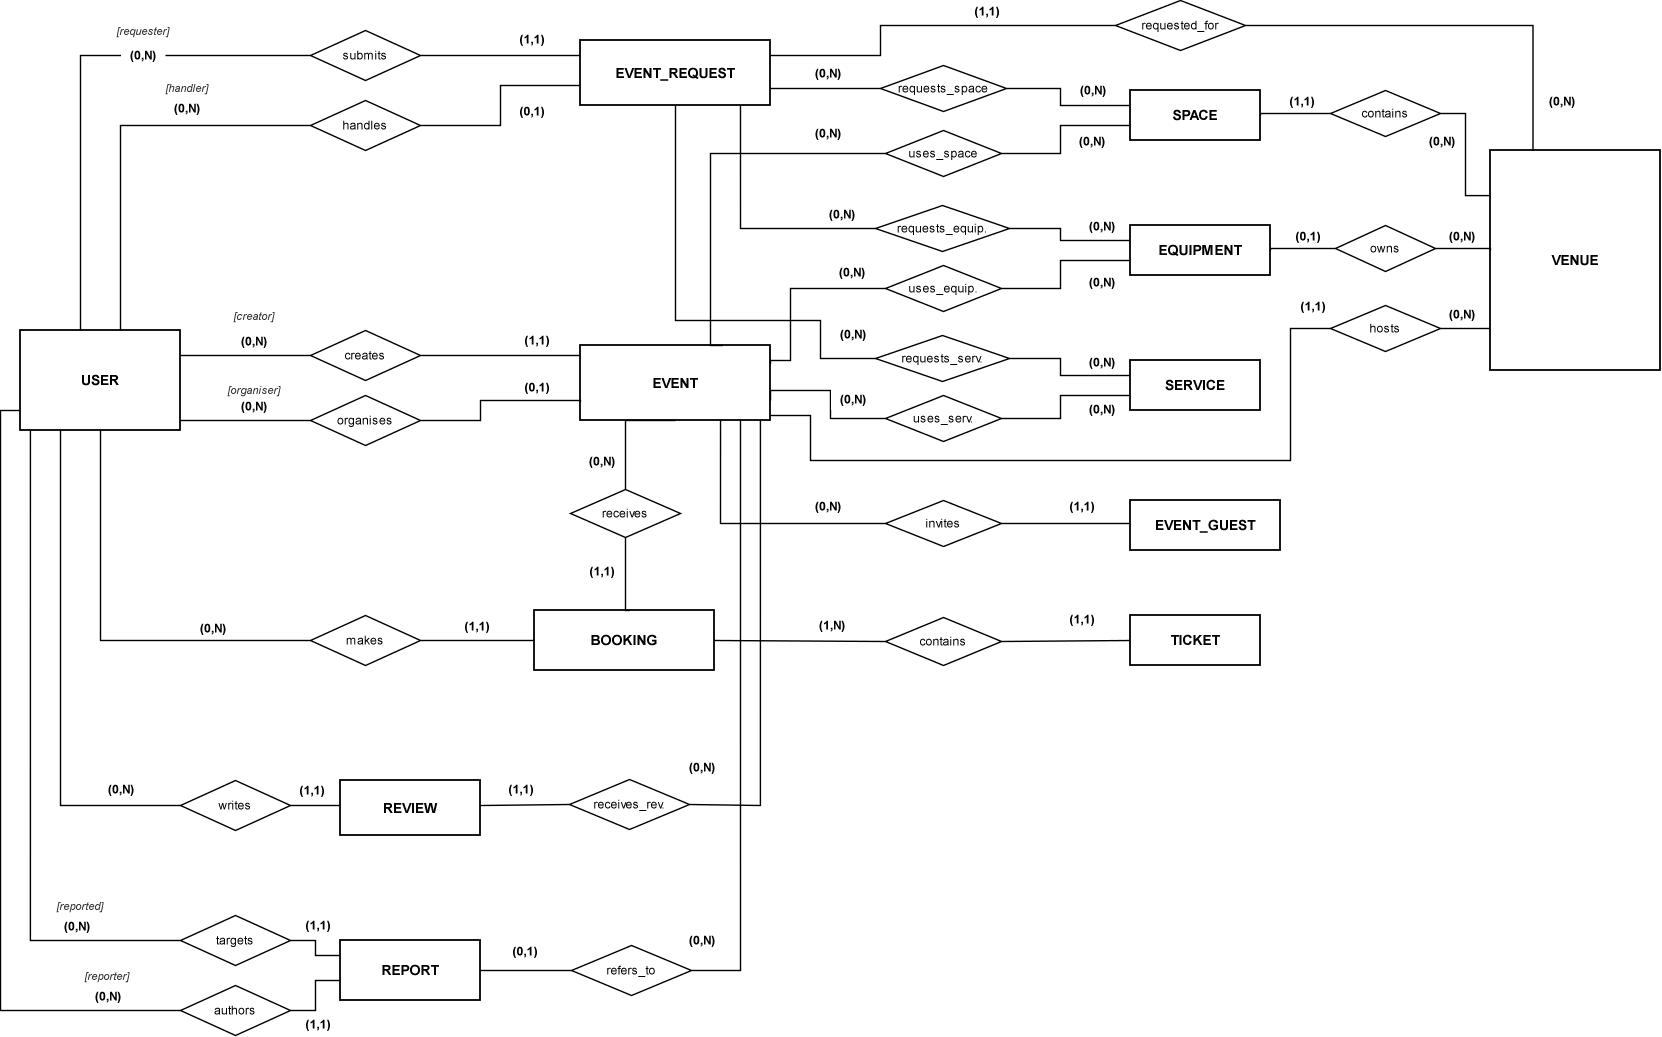
\includegraphics[width=\textwidth]{../docs/diagrams/database/entity-relationship-model.svg}
    \caption{Diagramma Entità-Relazione concettuale della base di dati.}
    \label{fig:er-diagram}
\end{figure}

\section{Modello relazionale}

Lo schema relazionale è costituito da 18 tabelle. La tabella seguente riassume gli attributi principali e i collegamenti tra entità; i tipi SQL e i vincoli sono definiti attraverso le migration Flyway.

\begin{table}[!htbp]
    \centering
    \renewcommand{\arraystretch}{1.25}
    \begin{tabular}{|p{0.31\textwidth}|p{0.63\textwidth}|}
        \hline
        \textbf{Tabella} & \textbf{Attributi e relazioni principali} \\
        \hline
        \texttt{USER} & Identificativo, username, hash della password (\texttt{password}), dati anagrafici e contatti, \texttt{is\_admin}, stato dell'account. \\
        \hline
        \texttt{VENUE} & Identificativo, nome, descrizione e indirizzo strutturato (\texttt{street}, \texttt{street\_number}, \texttt{city}, \texttt{postal\_code}, \texttt{country}, \texttt{additional\_info}). \\
        \hline
        \texttt{SPACE} & Identificativo, venue di appartenenza, nome e descrizione. \\
        \hline
        \texttt{EQUIPMENT} & Identificativo, eventuale venue, nome, descrizione e quantità totale (\texttt{total\_quantity}). \\
        \hline
        \texttt{SERVICE} & Identificativo, nome e descrizione. \\
        \hline
        \texttt{EVENT\_REQUEST} & Richiedente, handler facoltativo, venue, dati proposti, stato, timestamp di creazione e chiusura, preventivo facoltativo. \\
        \hline
        \texttt{EVENT} & Venue, creator, organiser facoltativo, dati descrittivi e temporali, capienza, stato, visibilità, prezzo e timestamp di pubblicazione. \\
        \hline
        \texttt{EVENT\_SPACE}, \texttt{REQ\_SPACE} & Tabelle associative per gli spazi collegati rispettivamente a eventi e richieste. \\
        \hline
        \texttt{EVENT\_EQUIPMENT}, \texttt{REQ\_EQUIPMENT} & Tabelle associative tra eventi o richieste e attrezzature; includono \texttt{quantity}. \\
        \hline
        \texttt{EVENT\_SERVICE}, \texttt{REQ\_SERVICE} & Tabelle associative tra eventi o richieste e servizi; includono \texttt{quantity}. \\
        \hline
        \texttt{BOOKING} & Utente, evento, timestamp di creazione, stato e prezzo totale (\texttt{total\_price}). \\
        \hline
        \texttt{TICKET} & Prenotazione di appartenenza, nominativo e inizio validità (\texttt{starts\_at}). \\
        \hline
        \texttt{EVENT\_GUEST} & Evento, dati dell'ospite invitato, stato e nota. \\
        \hline
        \texttt{REVIEW} & Utente autore, evento, valutazione, commento e timestamp di creazione. \\
        \hline
        \texttt{REPORT} & Utente segnalato, amministratore autore, evento facoltativo, severità, commento e timestamp di creazione. \\
        \hline
    \end{tabular}
    \caption{Riepilogo delle tabelle dello schema relazionale e dei relativi attributi principali.}
    \label{tab:tabelle-db}
\end{table}

Le relazioni uno-a-molti sono rappresentate da chiavi esterne nella tabella che dipende dall'altra entità. Le relazioni molti-a-molti sono invece tradotte in tabelle associative dotate di chiavi esterne verso le entità partecipanti.

Le tabelle associative degli spazi, dell'equipaggiamento e dei servizi definiscono chiavi primarie composte dalle due FK. La PK di \texttt{REQ\_EQUIPMENT} è estesa anche a \texttt{EVENT\_EQUIPMENT}, in modo da impedire duplicazioni della stessa attrezzatura all'interno di un medesimo evento.

L'indirizzo della venue è memorizzato tramite più colonne e non come tabella a sé: \texttt{street}, \texttt{street\_number}, \texttt{city}, \texttt{postal\_code}, \texttt{country} e \texttt{additional\_info}, con vincoli \texttt{NOT NULL} sui componenti essenziali dell'indirizzo.

Le chiavi esterne definiscono anche la gestione dell'eliminazione dei record. In alcuni casi la cancellazione dell'entità principale propaga l'eliminazione alle righe dipendenti, mentre in alcuni riferimenti facoltativi l'eliminazione del record referenziato imposta il campo a \texttt{NULL}. Le azioni referenziali variano sulle singole relazioni e non vanno intese come un comportamento uniforme a livello globale.

\section{Vincoli di integrità e regole applicative}

Lo schema utilizza chiavi primarie per identificare univocamente i record e chiavi esterne per garantire l'integrità referenziale. Sono inoltre presenti vincoli \texttt{NOT NULL}, valori predefiniti e vincoli \texttt{UNIQUE} o \texttt{CHECK} che operano direttamente a livello di database.

Tra i vincoli di tipo \texttt{CHECK} troviamo la quantità positiva nelle associazioni con le risorse, la capienza positiva degli eventi e la valutazione delle recensioni compresa tra 1 e 5. Le migration successive impongono inoltre che la data di fine di richieste ed eventi sia successiva a quella di inizio, che preventivo e prezzo non siano negativi quando valorizzati, che il prezzo totale di una prenotazione sia non negativo e che lo stato di pubblicazione risulti coerente con la presenza del timestamp \texttt{published\_at}, fatta eccezione per gli eventi cancellati.

L'unicità di username ed email è definita all'interno della tabella \texttt{USER}, e anche la coppia utente-evento di \texttt{REVIEW} è univoca, impedendo al medesimo utente di registrare più recensioni per lo stesso evento. Le tabelle associative impiegano chiavi primarie composte per evitare record duplicati.

Gli stati di account, richiesta, evento, prenotazione, ospite e severità del report sono rappresentati anche tramite tipi enumerativi PostgreSQL. I tipi enum limitano l'insieme dei valori memorizzabili, ma non definiscono le transizioni di stato ammesse.

Ulteriori regole di business sono demandate al livello applicativo. I service si occupano anche di verificare: che creator e handler siano amministratori e che l'organiser sia un utente ordinario; che una richiesta venga chiusa esclusivamente dall'handler assegnato; che una prenotazione riguardi un evento pubblicato, con visibilità pubblica e inizio futuro; che un account bannato non possa effettuare prenotazioni; che la creazione di una prenotazione richieda almeno un biglietto valido e verifichi la disponibilità dei posti nella stessa transazione, con precedente blocco dell'evento; che la pubblicazione di una recensione richieda che l'evento sia già concluso e che l'utente possieda una prenotazione confermata (garantito, oltre che dai service, anche dal vincolo presente sul database). Queste condizioni non sono interamente espresse da vincoli SQL e dipendono pertanto dai controlli eseguiti nei service.

\begin{table}[!htbp]
    \centering
    \renewcommand{\arraystretch}{1.25}
    \begin{tabular}{|p{0.25\textwidth}|p{0.69\textwidth}|}
        \hline
        \textbf{Livello di controllo} & \textbf{Vincoli e regole garantite} \\
        \hline
        \textbf{Database} \newline (vincoli SQL e PostgreSQL) &
        \textbf{Chiavi e integrità referenziale:} PK singole, PK composte sulle tabelle associative ed FK con azioni referenziali specifiche. \newline
        \textbf{Obbligatorietà e unicità:} vincoli \texttt{NOT NULL}, valori di default e vincoli \texttt{UNIQUE} su username ed email in \texttt{USER} e sulla coppia utente-evento in \texttt{REVIEW}. \newline
        \textbf{Vincoli \texttt{CHECK}:} quantità risorse e capienza eventi positive; valutazione recensioni tra 1 e 5; fine successiva all'inizio per eventi e richieste; preventivo, prezzo e totale prenotazione non negativi; coerenza tra stato pubblicato e \texttt{published\_at}. \newline
        \textbf{Tipi \texttt{ENUM}:} dominio ristretto dei valori ammessi per stati e livelli di severità. \\
        \hline
        \textbf{Applicativo} \newline (Service Layer) &
        \textbf{Ruoli e autorizzazioni:} verifica che creator e handler siano amministratori, che l'organiser sia un utente ordinario e che solo l'handler assegnato chiuda la richiesta. \newline
        \textbf{Prenotazioni e concorrenza:} controllo che l'evento sia pubblicato, pubblico e futuro, che l'utente non sia bannato, presenza di almeno un biglietto valido e verifica della capienza in transazione con blocco preventivo dell'evento. \newline
        \textbf{Recensioni e transizioni:} verifica che l'evento sia concluso e l'utente abbia una prenotazione confermata; controllo delle transizioni di stato ammesse tra gli enum. \\
        \hline
    \end{tabular}
    \caption{Suddivisione dei vincoli tra livello di persistenza e livello applicativo.}
    \label{tab:vincoli-db-app}
\end{table}

\section{Evoluzione dello schema}

L'evoluzione dello schema è gestita tramite script SQL versionati con Flyway nella directory \texttt{src/main/resources/db/migration}. Le migration sono eseguite in ordine sequenziale e descrivono sia la creazione iniziale di tipi e tabelle sia le modifiche incrementali successive. Il loro contenuto documenta l'evoluzione progettata per lo schema, pur non costituendo da solo prova dell'avvenuta applicazione su uno specifico ambiente.

Le prime migration creano i tipi enumerativi, le tabelle principali, le risorse, le richieste e gli eventi; seguono le tabelle associative, le prenotazioni, gli invitati e gli elementi di feedback. Le migration successive consolidano e completano lo schema: \texttt{V10} struttura l'indirizzo della venue e introduce il prezzo totale nella prenotazione; \texttt{V11} corregge il nome di una colonna; \texttt{V12} e \texttt{V13} introducono lo stato iniziale \texttt{DRAFT}; \texttt{V14} impone l'unicità delle recensioni per coppia utente-evento; \texttt{V15} consolida i campi obbligatori dell'indirizzo; \texttt{V16} aggiunge vincoli di coerenza sul dominio; \texttt{V17} completa la chiave primaria di \texttt{EVENT\_EQUIPMENT}.

La migration \texttt{V9} contiene dati iniziali destinati all'ambiente di sviluppo; tali record sono distinti dalla definizione strutturale dello schema e non vanno considerati dati di produzione. Le migration già rilasciate e applicate non devono essere modificate retroattivamente: qualsiasi evoluzione futura va introdotta tramite una nuova migration versionata.